%
% $RCSfile: information_processing_model.tex,v $
%
% Copyright (C) 2002-2008. Christian Heller.
%
% Permission is granted to copy, distribute and/or modify this document
% under the terms of the GNU Free Documentation License, Version 1.1 or
% any later version published by the Free Software Foundation; with no
% Invariant Sections, with no Front-Cover Texts and with no Back-Cover
% Texts. A copy of the license is included in the section entitled
% "GNU Free Documentation License".
%
% http://www.cybop.net
% - Cybernetics Oriented Programming -
%
% http://www.resmedicinae.org
% - Information in Medicine -
%
% Version: $Revision: 1.1 $ $Date: 2008-08-19 20:41:07 $ $Author: christian $
% Authors: Christian Heller <christian.heller@tuxtax.de>
%

\subsection{Information Processing Model}
\label{information_processing_model_heading}
\index{Information Processing Model}
\index{Chunking}

Information processing, from the view of \emph{Cognitive Psychology}, follows
the model shown in figure \ref{processing_figure}. General information has to
pass several stages before it becomes meaningful knowledge. The results of
processing stages are stored in different memories.

\begin{figure}[ht]
    \begin{center}
        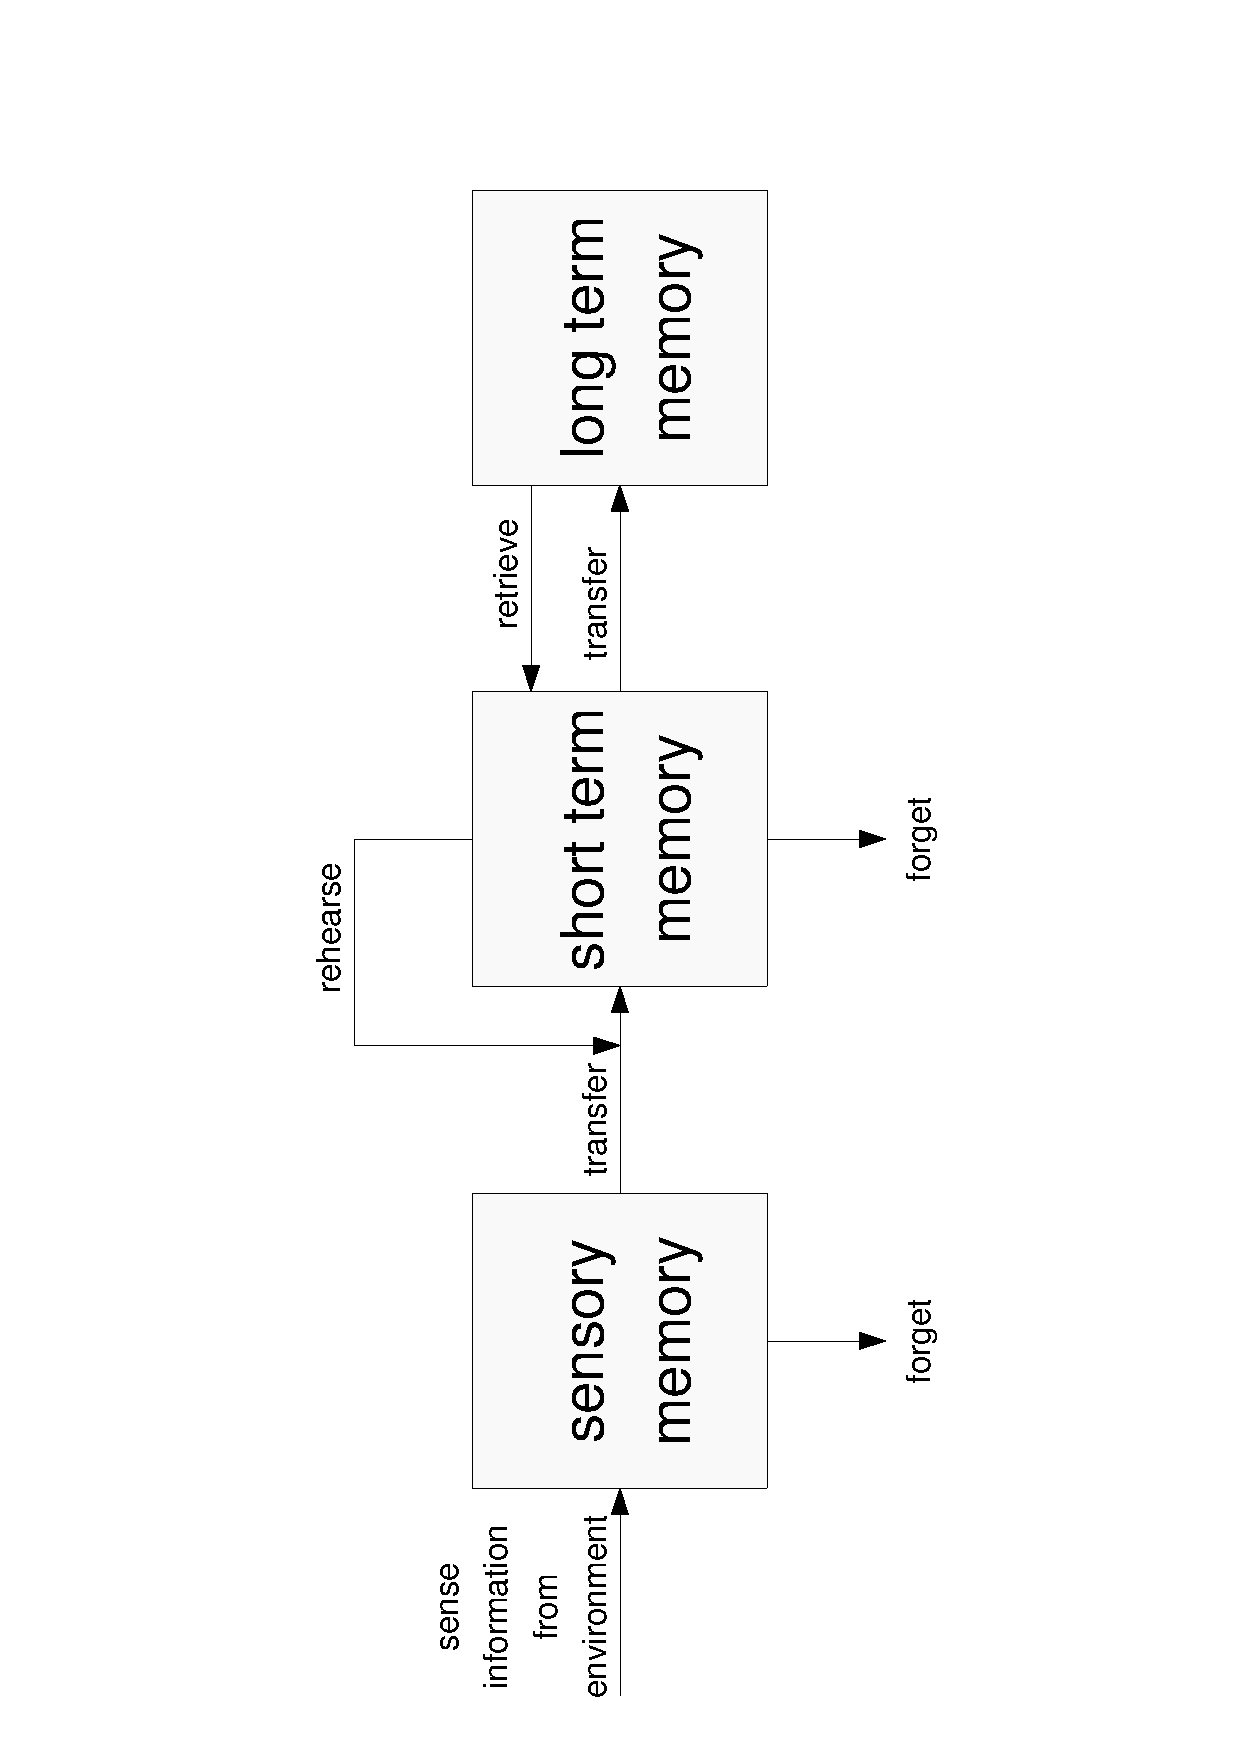
\includegraphics[scale=0.3,angle=-90]{graphic/processing.pdf}
        \caption{Information Processing Model \cite{eet}}
        \label{processing_figure}
    \end{center}
\end{figure}

The \emph{Encyclopedia of Educational Technology} (EET) \cite{eet} writes on
this:

\begin{quote}
    After entering sensory memory, a limited amount of information is
    transferred into short-term memory. \ldots\ The process of transferring
    information from STM into LTM involves the \emph{Encoding} or
    \emph{Consolidation} of information. \ldots\ Recent research (focuses) on
    the necessity of the brain to organise complex information in STM
    \emph{before} it can be encoded into LTM.

    In this process of organization, the \emph{Meaningfulness} or
    \emph{Emotional Content} of an item may play a greater role in its
    retention into LTM. Also, on a more concrete level, the use of
    \emph{Chunking} has been proven to be a significant aid to STM transfer to
    LTM. Because STM's capacity is limited to seven items, regardless of the
    complexity of those items, chunking allows the brain to automatically group
    certain items together.
\end{quote}

Certainly, the emotional content of an item can be neglected for computer
systems as of today. But chunking as a technique to divide information into
discrete items is of great importance in human thinking, which gets
investigated closer in chapter \ref{knowledge_schema_heading}.
